\documentclass[10pt]{article}
\usepackage[margin=21mm]{geometry}
\usepackage{amsmath,amssymb,graphicx,booktabs,enumitem,xcolor}
\usepackage[colorlinks=true,urlcolor=blue!55!black,linkcolor=blue!55!black]{hyperref}
\setlength{\parindent}{0pt}\setlength{\parskip}{5pt}
\setlist{nosep,leftmargin=*}\setlength{\emergencystretch}{2em}
\graphicspath{{figures/}}
\begin{document}
\begin{center}
{\LARGE SIR fit to mouse pathology}\\[5pt]
{\large Baseline, diagnosis and explicit extensions}\\[4pt]
\small 27 November 2026. Exploratory fits to the existing cohort.
\end{center}

\section*{The model}
A cell moves $S\to I\to R$. Removed cells cannot transmit, cannot be infected again, and contribute nothing to the pathology readout. $R$ can represent death or lasting resistance; the measurements do not distinguish them.

At reference voxel $i$, $S_i+I_i+R_i=N_i$. The exact count CTMC has transitions
\begin{align*}
(S_i,I_i,R_i)&\longrightarrow(S_i-1,I_i+1,R_i), &
\lambda_i&=\chi_i\frac{S_i}{N_i}\sum_j(\beta_TQ_{ji}+\beta_LL_{ji})I_j,\\
(S_i,I_i,R_i)&\longrightarrow(S_i,I_i-1,R_i+1), &
\mu_i&=\gamma_i I_i.
\end{align*}
The uniform baseline has $\chi_i=1$ and $\gamma_i=\gamma$. $Q$ and $L$ have sources in rows. Rates have units month$^{-1}$; $\chi_i$ is dimensionless. $N_i$, tissue volume and contacts remain fixed after removal. Initial $R_i=0$.

The reference is unchanged: 448,962 voxels of side $100\,\mu$m and 39,476,440 estimated neurons. $Q$ is the cell-reversed Allen tracer-derived operator, $D^{-1}W^TD/c$ with $D=\operatorname{diag}(N)$ and $c=24.3813178615$. $W$ is the released, interpolated voxel connectivity model, not independently measured probabilities for every voxel pair. The local channel has $L_{ji}\propto N_i\exp[-d_{ji}^2/(2\sigma^2)]$, $\sigma=200\,\mu$m and cutoff $600\,\mu$m. Its rows sum to one and include $i=j$.

\section*{The observation rule}
We retain 18,292 cell-body profile-density records from 55 mice at 0.1, 0.2, 0.3, 0.5, 1, 3, 6 and 9 months. Different times contain different mice. Observed zeros are retained; missing observations are not replaced by zeros.
\[
\widehat y_r=10^6 h[O\,\mathbb E I(t_r)]_{g(r)},\qquad h=6\,\mu\mathrm m.
\]
$O$ maps voxel counts to mean density per $\mu$m$^3$ in the corresponding anatomical window; predictions are profiles/mm$^2$. Only $I$ contributes. This is immediate ideal cell-center counting in a 6-$\mu$m section, with representative regional sampling. It is an explicit approximation: object extent, detection and actual section coverage have not been reconstructed. There is no fitted amplitude or pathology delay in these experiments.

\section*{Comparison}
For either set of weights, we minimize
\[
J=\frac{\sum_r w_r[\widehat y_r-y_r]^2}{\sum_r w_ry_r^2}
\]
and report $\sqrt J$. Zero prediction scores one. The original weights normalize reported area proxies within each mouse, then give equal weight to mice within a time and to the eight times. The sensitivity analysis gives equal weight to regional records within each mouse instead. Both scores are reported for every completed reference check. They are different objectives, not interchangeable measures of improvement.

\newpage
\section*{Completed reference checks}
The best completed reference check reduces the original relative RMS error from 0.9180 to 0.8694, a 10.3\% reduction in weighted squared error. Its Monte Carlo standard error is 0.00009; this quantifies simulation noise only. The trajectories still miss important regional peaks. This is an improved fit, not a successful explanation of the whole dataset.

The revised initial state has expected burden $B=21511.1$ and tracer-footprint fraction $f=0.8385$. These are fitted assumptions about an unobserved starting state, not measured counts of initially affected cells.

\begin{center}\small\begin{tabular}{lrrr}\toprule Model & Area-weighted RMS & Equal-region RMS & Paths\\\midrule
Uniform SIR & 0.9180 & 0.9641 & 512\\
Revised initial state & 0.8969 & 0.9438 & 64\\
Composition rates, area fit & 0.8829 & 0.9341 & 64\\
Composition rates, regional fit & 0.8694 & 0.9106 & 128\\
\bottomrule\end{tabular}\end{center}
These are in-sample comparisons on the same mouse observations. Fresh CTMC paths assess simulation noise, not validation on new animals. The composition candidates are finite-budget search results, not established global optima. The figure uses the completed candidate with the lowest original area-weighted error.

\begin{figure}[h]
\centering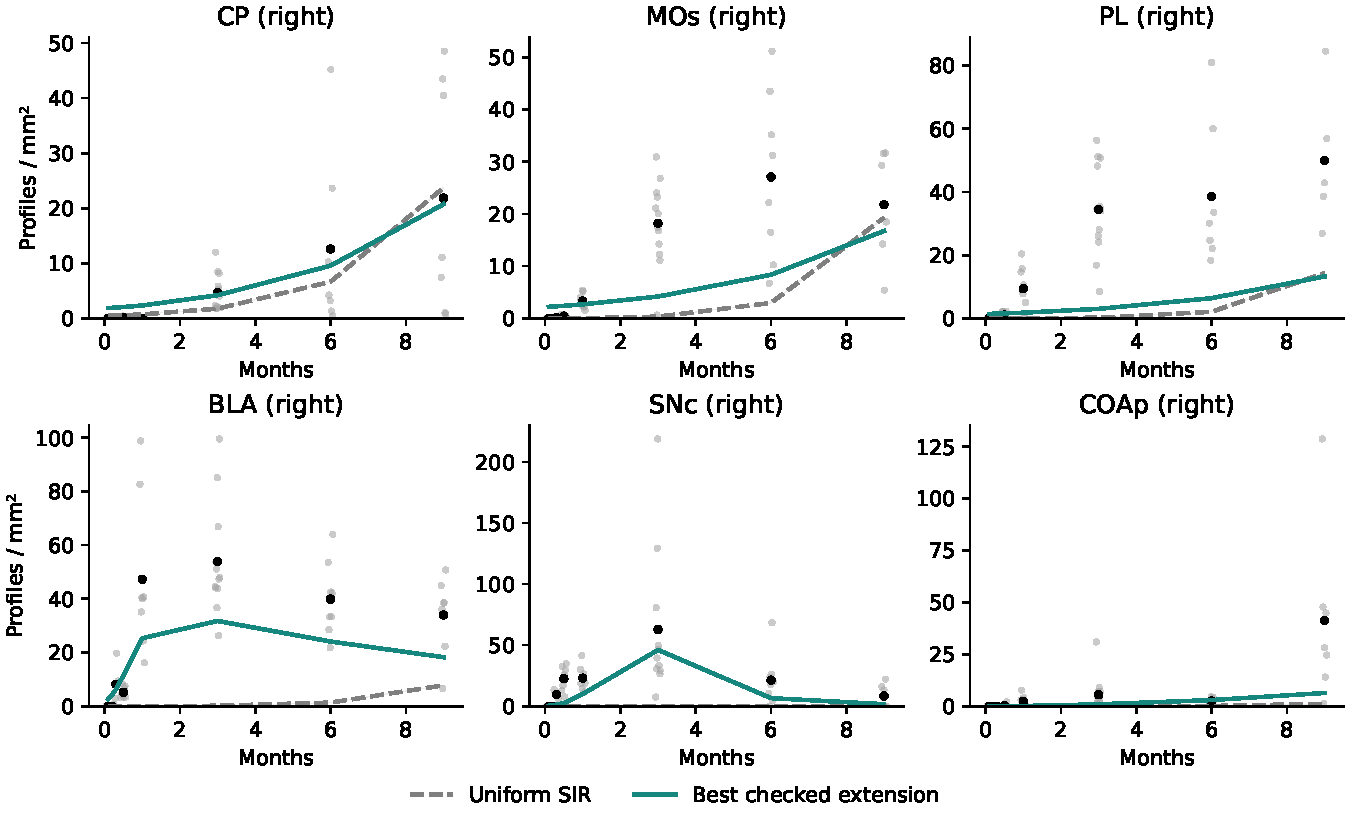
\includegraphics[width=\linewidth]{sir_initial_comparison.pdf}
\caption{Full 100-$\mu$m CTMC ensemble means. Gray dots are individual mice and black dots are their arithmetic means for each plotted region and time. Shading is $\pm1.96$ Monte Carlo standard errors of the simulated mean; it does not represent animal variability or parameter uncertainty. All regions shown are right-sided.}
\end{figure}

\newpage
\section*{What changed, and what did not help}
\textbf{Wider uniform-rate searches.} The original direct CTMC search used rates in $[0,1]$/month, three starts and 80 evaluations per start. A later 800-$\mu$m deterministic screen searched $10^{-4}$--30/month with differential evolution and local refinement. Separate searches fixed removal at 0.1, 1, 5 and 20/month and parameterized the remaining rates through the coarse dilute growth exponent. Neither screen produced a material improvement in its uniform-model fit. These are coarse search results, not an exhaustive rejection of every full-resolution parameter set.

\textbf{Initial state.} The original seed was a provisional 1,000-cell focus in right caudoputamen. Let $p^{\rm loc}=I^{\rm old}(0)/1000$ and
\[
p^{\rm proj}=\frac{Q^Tp^{\rm loc}}{\boldsymbol 1^TQ^Tp^{\rm loc}}.
\]
The new initial-state hypothesis is
\[
I_i(0)\sim\operatorname{Binomial}\left(N_i,\frac{B[(1-f)p_i^{\rm loc}+fp_i^{\rm proj}]}{N_i}\right)
\]
independently across voxels. $B$ is the expected initial burden. Candidate probabilities exceeding one are rejected. This represents unresolved early uptake/transport to projecting neurons. The footprint uses the frozen tracer and population, not pathology-derived destination weights. It is not a registered or measured initial infection. Rates, $B$ and $f$ were fitted jointly in the coarse screen; fresh full-reference paths then checked the candidate. Subsequent composition tests held this initial law fixed.

\textbf{Composition-dependent rates.} MERFISH provides three fractions: $f_{iO}$ for other or unknown neurons, $f_{iG}$ for glutamatergic neurons and $f_{iD}$ for dopamine/serotonin neurons. They sum to one. We tested
\[
\chi_i=f_{iO}+q_Gf_{iG}+q_Df_{iD},\qquad
\gamma_i=\gamma_Of_{iO}+\gamma_Gf_{iG}+\gamma_Df_{iD}.
\]
These are voxel environment-dependent rates: every cell in a voxel still shares them. They are \emph{not} a cell-type-stratified simulation. The reference contact matrices are not renormalized. Seven shared parameters replace the three uniform rates. Search used 1,265 anatomical compartments, retaining each originally seeded voxel separately; target-weighted contacts and the observation operator were aggregated from the reference. Five stated starts were tested. The equal-region sensitivity continued from those endpoints, and three additional high-susceptibility starts were screened. Exact full-reference checks remain distinct from these ODE searches.

\textbf{Data and construction audit.} The local voxel ordering and hemisphere split agree with the published Allen mask implementation. One observation exceeds the maximum density permitted by the 6-$\mu$m rule; the error forced by that ceiling is only 0.0087 in relative RMS, so it cannot explain the poor overall fit. Giving each anatomical window its own fitted amplitude still leaves relative RMS 0.8052 for the original SIR trajectory. This is a diagnostic overfit, not a proposed observation model. Timing and regional distribution remain problems.

\newpage
\section*{Error and limitations}
\begin{figure}[h]
\centering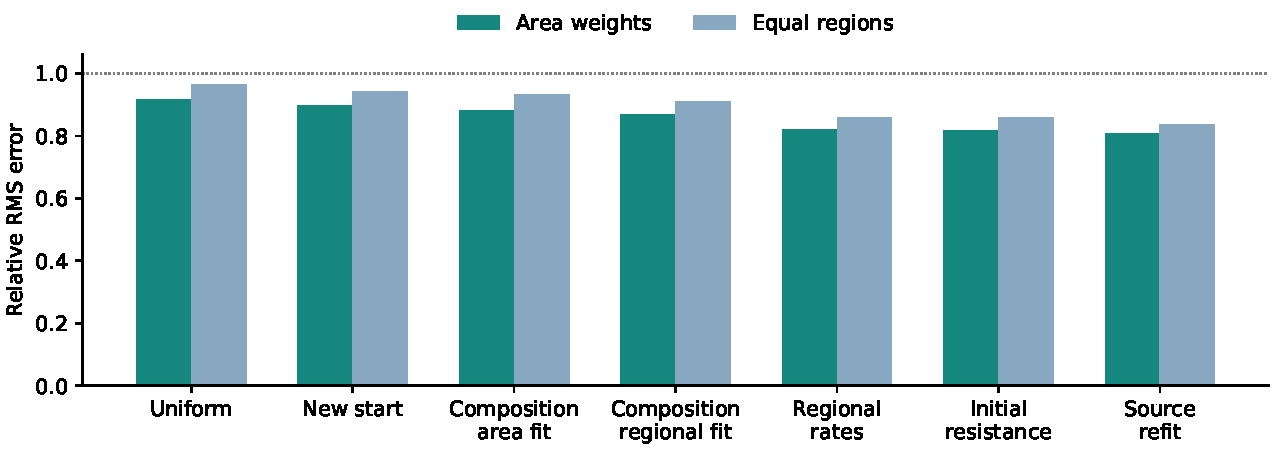
\includegraphics[width=.85\linewidth]{fit_errors.pdf}
\caption{All completed candidates scored under both weighting rules. The dotted line is zero prediction. Different weights change which discrepancies matter; a lower score under a new weighting rule alone is not evidence of improvement under the old rule.}
\end{figure}
\begin{figure}[h]
\centering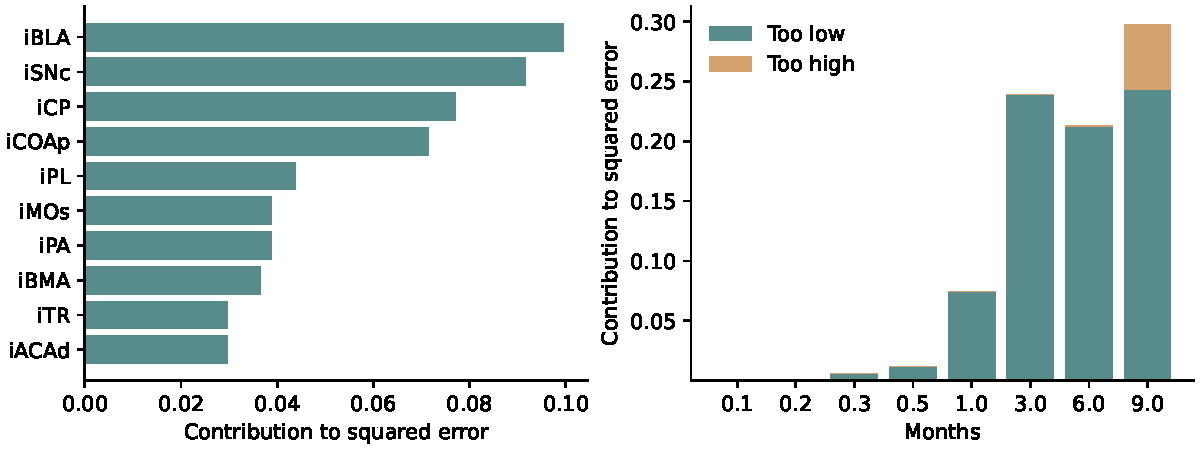
\includegraphics[width=\linewidth]{error_diagnosis.pdf}
\caption{Where the original uniform SIR fit fails. Left: the largest regional contributions to its original weighted squared error. Right: contributions by time, separated into underprediction and overprediction. The prefix ``i'' denotes the ipsilateral/right side.}
\end{figure}

The changes produce measurable improvement but do not establish a satisfactory model of the observed propagation. In particular, a global error can improve while early amygdala and substantia nigra peaks remain poorly described. More simulation precision cannot remove that discrepancy. Large or poorly constrained fitted rate differences should not be interpreted as measured biological susceptibilities or lifetimes.

The sampled tissue operator, initial exposure and correspondence between tracer signal and cell-to-cell transfer remain assumptions. Registered section masks and raw count/area checkpoints would allow a more faithful measurement comparison. The current positive-coordinate exports alone do not establish sampled tissue with zero pathology. No missing tissue masks or calibrated detection model were invented for this report.

\section*{Reproduction and validation}
The checked parameter sets are below. Rates are in month$^{-1}$; $q_G$ and $q_D$ are dimensionless. Uniform models repeat the same removal rate in the three columns. These are conditional fitted coefficients, not independently measured biological constants.
\begin{center}\scriptsize\begin{tabular}{lrrrrrrr}\toprule Model & $\beta_T$ & $\beta_L$ & $\gamma_O$ & $q_G$ & $q_D$ & $\gamma_G$ & $\gamma_D$\\\midrule
Uniform & 0.134 & 0.465 & 0.00372 & 1 & 1 & 0.00372 & 0.00372\\
New start & 0.000414 & 0.295 & 0.0102 & 1 & 1 & 0.0102 & 0.0102\\
Composition (area) & 0.0277 & 0.408 & 0.0677 & 2.6 & 10.8 & 0.84 & 2.48\\
Composition (regions) & 0.618 & 0.57 & 0.343 & 0.13 & 0.0268 & 0.0359 & 3.66e-05\\
Regional rates & 0.335 & 0.233 & 0.0423 & 0.365 & 0.0102 & 0.0544 & 7.81e-05\\
Initial resistance & 0.208 & 0.298 & 0.0629 & 0.667 & 0.0103 & 0.17 & 3.45e-05\\
Source refit & 0.281 & 0.2 & 0.0752 & 0.426 & 0.0101 & 0.0387 & 9.67e-05\\
\bottomrule\end{tabular}\end{center}
The last row's small susceptibility and removal coefficients in dopamine/serotonin-rich voxels do not explain the observed substantia nigra peak. This is one reason the best global score must not be treated as biological validation.

The adjacent README lists commands and output folders. \texttt{metrics.json} contains both scores and Monte Carlo standard errors. Each simulation saves rates, seeds, event counts, infected and removed means, and the explicit initial/rate fields when used. The full-reference input hashes are fixed by the existing model report and baseline configuration. The extension implementation is recorded in commit \texttt{21c7789}.

The stochastic transitions were checked against an independently assembled finite-state SIR generator, including nonuniform susceptibility and removal. The positive ODE integrator was checked against an independent high-accuracy solver. The local composition aggregation was checked by explicit enumeration. The original reference SIS trajectories remain bitwise unchanged when the new options are omitted. These validate implementation of the stated model, not its biological adequacy.

\small
Sources: \href{https://doi.org/10.1101/2024.10.22.619411}{pathology study}; \href{https://doi.org/10.1162/netn_a_00066}{Knox et al. voxel connectivity model}; \href{https://github.com/AllenInstitute/mouse_connectivity_models/blob/7637e405d7d97bea4b82758c18e825651f4a7815/mcmodels/core/masks.py}{pinned Allen mask code}. Full data provenance and earlier assumptions are in the \href{https://github.com/gretarsson/pixel-sis/blob/main/docs/report/pixel_sis_report.pdf}{original model report}.
\end{document}
